\section{Current replication object}
R24 contains thirty tuning trajectories, twenty-eight held-out trajectories, thirty-six multicell trajectories, twelve reference trajectories and four post-hoc failure trajectories. All 110 are retained. There are 286 prescribed checkpoint records, of which 140 belong to the central held-out experiment. These categories are not pooled to inflate the number of independent replications.

\subsection{Chronology and the operational repair}
Protocol commit \path{b54afa8c9107d70094a1d84be4a3c0279916530c} precedes the scientific execution. Primary run \path{35832563885} completed all tuning, held-out and multicell computations. It then stopped while strict JSON encoded an unused financing-root diagnostic as infinity in the reference economy, which has no financing equation. The exact metadata patch encodes the unused nonfinite value as null; it changes no objective, seed, rate, checkpoint, policy or certificate.

The full primary archive is retained at \path{archive/primary_execution.zip}, SHA-256 \path{cf8da93098d0e32c6d6bd219e57aedc84a9b31d1adbee941a004a85d2a44cde8}. Recovery run \path{35833755321} restored this archive, did not repeat or select among primary trajectories, and completed only the reference and failure stages. Every primary result was checked byte-identical. Failed execution, source identity and correction are preserved. Reference/failure stages used a separately provisioned machine; cross-stage times are not controlled same-machine comparisons.

Every pre-existing file from the reviewed branch is checked against its Git blob identifier in the publication audit. All new evidence and manuscripts are confined to R24 paths. The preceding main-text and supplement components remain in the new manuscripts with explicit historical notices; their revision-specific observations do not override the R24 domains.

\subsection{Analytical hypotheses and numerical instantiations}
\begin{table}[htbp]\centering\small
\caption{Dependency map for the current claims}
\begin{tabularx}{\textwidth}{lXX}\toprule
Claim & Analytical assumptions & Executed evidence\\\midrule
State realization & Common observed factor; constant weights; conditional-price identity; positive accounts; common shocks. & Frozen expert coefficients and the unchanged financing/feasibility checker.\\
Augmented value & Original full Brownian filtration; causal memory; identical actions and stopping; admissible concatenation. & Analytical theorem, not a numerical full-state accuracy claim.\\
Regional regret & Joint concavity on the actual range; shared shocks; convex explicit upper; uniform nonsynchronized exit allowance. & Nine actual experts per arm, every cell, directed vertex certificates.\\
Payoff replacement & New lower bound strictly exceeds old upper bound at identical initialization. & Every replayed acceptance and rejection.\\
Output geometry & Differentiability and local Jacobian Lipschitz continuity for the Taylor remainder. & Actual Jacobian and adaptive-metric spectra and transport remainders; ordinary diagnostics.\\
Gradient error & Common price bracket; positive price derivative; derivative approximation and offset-Lipschitz bounds. & Conditional theorem; ordinary quadrature differences do not instantiate a rigorous stopped-gradient bound.\\
Reference gap & Deterministic reference; exact constant optimum in both continuous parameter classes. & Directed reference/candidate intervals and exact slab integration.\\\bottomrule
\end{tabularx}\end{table}

\section{Complete cost accounting}
\begin{table}[htbp]\centering\footnotesize\setlength{\tabcolsep}{4pt}
\caption{Standalone costs, instrumentation and upper-library allocation}\label{tab:r24cost}
\begin{tabular}{llrrrrrr}\toprule
Rule & Arm & Prep. & Initial & Diag. & Cert. & + dual & Tune\\\midrule
8/16 & Neural--Adam & 0.000 & 2.063 & 0.127 & 13.744 & 429.533 & 16.364\\
8/16 & Direct--Adam & 0.000 & 2.063 & 0.111 & 13.656 & 429.445 & 15.942\\
8/16 & Diagonal--Adam & 0.002 & 2.063 & 0.111 & 13.574 & 429.363 & 16.062\\
8/16 & Tangent--Adam & 0.002 & 2.063 & 0.112 & 13.573 & 429.362 & 15.991\\
8/16 & Whitened--Adam & 0.002 & 2.063 & 0.111 & 13.617 & 429.406 & 15.927\\
8/16 & Neural--L-BFGS-B & 0.000 & 2.063 & 0.110 & 13.333 & 429.122 & 0.000\\
8/16 & Direct--L-BFGS-B & 0.000 & 2.063 & 0.105 & 12.784 & 428.573 & 0.000\\
12/24 & Neural--Adam & 0.000 & 2.060 & 0.125 & 14.427 & 430.216 & 16.364\\
12/24 & Direct--Adam & 0.000 & 2.060 & 0.111 & 14.272 & 430.061 & 15.942\\
12/24 & Diagonal--Adam & 0.002 & 2.060 & 0.110 & 14.253 & 430.042 & 16.062\\
12/24 & Tangent--Adam & 0.002 & 2.060 & 0.110 & 14.286 & 430.075 & 15.991\\
12/24 & Whitened--Adam & 0.002 & 2.060 & 0.113 & 14.420 & 430.209 & 15.927\\
12/24 & Neural--L-BFGS-B & 0.000 & 2.060 & 0.111 & 13.722 & 429.511 & 0.000\\
12/24 & Direct--L-BFGS-B & 0.000 & 2.060 & 0.106 & 13.037 & 428.826 & 0.000\\
\bottomrule\end{tabular}
\par\smallskip\begin{minipage}{.97\textwidth}\footnotesize Seconds. Diag. is additional optional scientific instrumentation. Cert. includes generation, preprocessing, initial and checkpoint checking. + dual adds the unamortized historical 415.789-second construction; divide that charge by M for M valid reuses. Tune charges all tuning trials and is additional. The historical dual charge is not a same-machine timing comparison.\end{minipage}
\end{table}

Generator-only curves exclude scientific instrumentation. Certified-solve cost includes preprocessing, initial checking and every checkpoint check. Instrumentation, tuning and the historical upper library are additional and separately listed. Shared initial policies and initial geometry can be reused, but standalone columns conservatively charge each method. Their sum is not presented as the measured wall time of the shared study. The dual reuse allocation is valid only when the same unrestricted library remains applicable to the economy.

\section{Certified checkpoint curves}
Each curve includes caps 25, 50, 100, 200 and 400. For line-search methods, the most recent accepted iterate available by the cap is used; terminated endpoints retain actual calls. The ordinate's maximum across two seeds is an envelope of two certified problems, not a confidence interval. Snapshots were archived prospectively and checked serially afterward. The cumulative certification axis reconstructs the specified checking schedule, not an online rollback experiment.
\begin{figure}[p]\centering
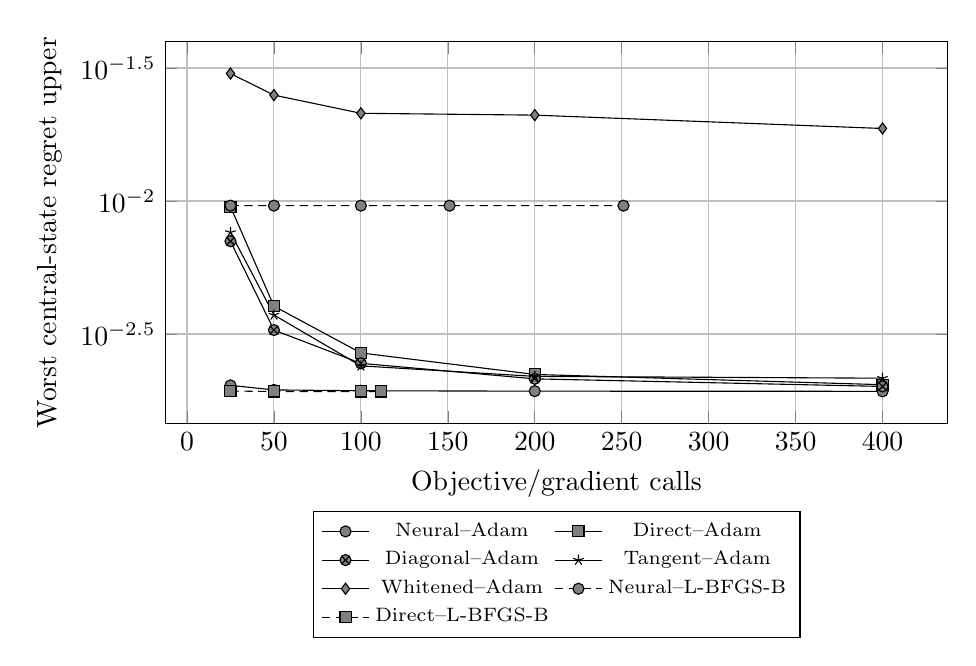
\begin{tikzpicture}\begin{axis}[width=.95\textwidth,height=.53\textwidth,ymode=log,xlabel={Objective/gradient calls},ylabel={Worst central-state regret upper},legend style={font=\scriptsize,at={(0.5,-0.23)},anchor=north,legend columns=2},cycle list name=black white,grid=major]
\addplot+ coordinates {(25,0.00202746061517) (50,0.00194950145597) (100,0.0019349101657) (200,0.00192863167763) (400,0.00192571291215)};\addlegendentry{Neural--Adam}
\addplot+ coordinates {(25,0.0095266270982) (50,0.00402455251775) (100,0.00268452213393) (200,0.00222821354893) (400,0.00203922705228)};\addlegendentry{Direct--Adam}
\addplot+ coordinates {(25,0.00706010753057) (50,0.00327282233924) (100,0.00245383492174) (200,0.00214493939263) (400,0.00200873460523)};\addlegendentry{Diagonal--Adam}
\addplot+ coordinates {(25,0.00761882459032) (50,0.00372955082102) (100,0.00239992613935) (200,0.00219163615955) (400,0.00215723161614)};\addlegendentry{Tangent--Adam}
\addplot+ coordinates {(25,0.0301532988188) (50,0.025022949821) (100,0.0213764994292) (200,0.0210368831176) (400,0.0187420285412)};\addlegendentry{Whitened--Adam}
\addplot+ coordinates {(25,0.00960967109684) (50,0.00960832614177) (100,0.00960832614177) (151,0.00960832614177) (251,0.00960832614177)};\addlegendentry{Neural--L-BFGS-B}
\addplot+ coordinates {(25,0.00193054208314) (50,0.00192368858146) (100,0.00192344285797) (111.5,0.00192344285797) (111.5,0.00192344285797)};\addlegendentry{Direct--L-BFGS-B}
\end{axis}\end{tikzpicture}
\caption{All five prospective checkpoints, rule 8/16. Ordinate: worse regret bound across two seeds; abscissa: mean actual calls or cost. Lines connect recorded checkpoints, not extra observations. Certification is serial replay, so cumulative cost is reconstructed rather than directly timed online wall time.}\end{figure}
\begin{figure}[p]\centering
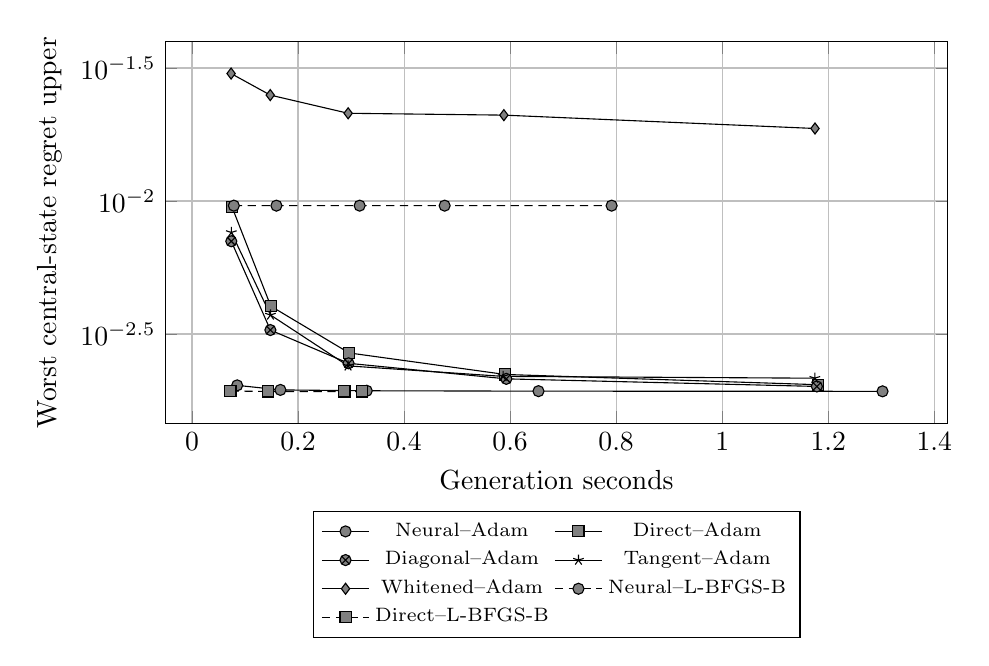
\begin{tikzpicture}\begin{axis}[width=.95\textwidth,height=.53\textwidth,ymode=log,xlabel={Generation seconds},ylabel={Worst central-state regret upper},legend style={font=\scriptsize,at={(0.5,-0.23)},anchor=north,legend columns=2},cycle list name=black white,grid=major]
\addplot+ coordinates {(0.085190371,0.00202746061517) (0.1667503465,0.00194950145597) (0.3295984665,0.0019349101657) (0.653513655,0.00192863167763) (1.302440713,0.00192571291215)};\addlegendentry{Neural--Adam}
\addplot+ coordinates {(0.075180235,0.0095266270982) (0.1486825755,0.00402455251775) (0.296327056,0.00268452213393) (0.5904344295,0.00222821354893) (1.180453165,0.00203922705228)};\addlegendentry{Direct--Adam}
\addplot+ coordinates {(0.0740899265,0.00706010753057) (0.1478579445,0.00327282233924) (0.29530931,0.00245383492174) (0.592865943,0.00214493939263) (1.178593873,0.00200873460523)};\addlegendentry{Diagonal--Adam}
\addplot+ coordinates {(0.074168682,0.00761882459032) (0.1480145975,0.00372955082102) (0.294343687,0.00239992613935) (0.5867250355,0.00219163615955) (1.174718289,0.00215723161614)};\addlegendentry{Tangent--Adam}
\addplot+ coordinates {(0.0737032085,0.0301532988188) (0.1476078865,0.025022949821) (0.294509208,0.0213764994292) (0.5882263245,0.0210368831176) (1.1750650195,0.0187420285412)};\addlegendentry{Whitened--Adam}
\addplot+ coordinates {(0.0789034485,0.00960967109684) (0.1592275735,0.00960832614177) (0.3161687915,0.00960832614177) (0.476508957,0.00960832614177) (0.791457727,0.00960832614177)};\addlegendentry{Neural--L-BFGS-B}
\addplot+ coordinates {(0.0725573095,0.00193054208314) (0.143977069,0.00192368858146) (0.287535419,0.00192344285797) (0.320645736,0.00192344285797) (0.320645736,0.00192344285797)};\addlegendentry{Direct--L-BFGS-B}
\end{axis}\end{tikzpicture}
\caption{All five prospective checkpoints, rule 8/16. Ordinate: worse regret bound across two seeds; abscissa: mean actual calls or cost. Lines connect recorded checkpoints, not extra observations. Certification is serial replay, so cumulative cost is reconstructed rather than directly timed online wall time.}\end{figure}
\begin{figure}[p]\centering
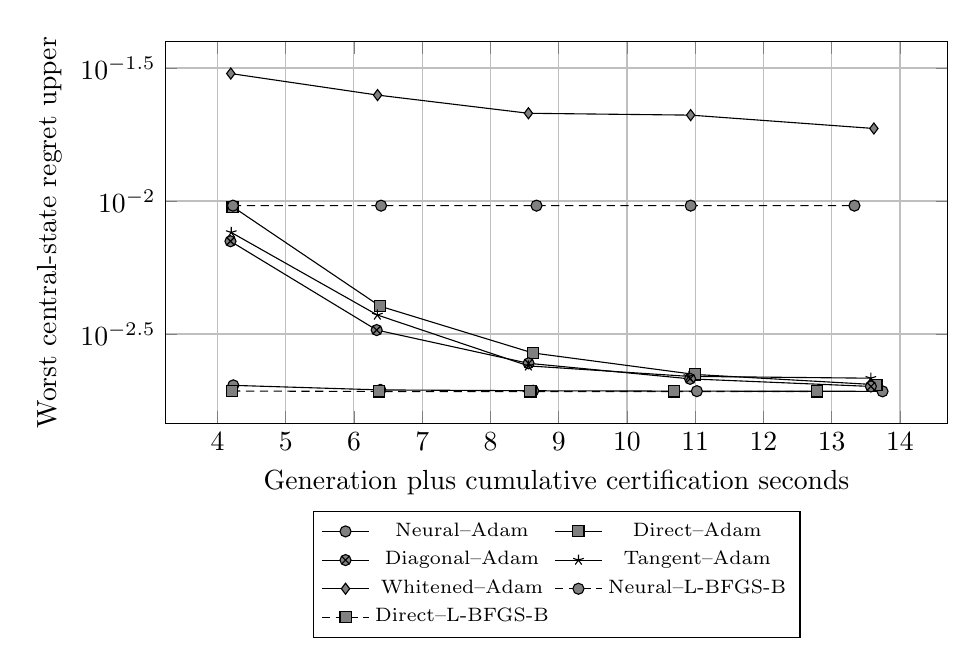
\begin{tikzpicture}\begin{axis}[width=.95\textwidth,height=.53\textwidth,ymode=log,xlabel={Generation plus cumulative certification seconds},ylabel={Worst central-state regret upper},legend style={font=\scriptsize,at={(0.5,-0.23)},anchor=north,legend columns=2},cycle list name=black white,grid=major]
\addplot+ coordinates {(4.2325075875,0.00202746061517) (6.38725457,0.00194950145597) (8.6262041475,0.0019349101657) (11.024284957,0.00192863167763) (13.744141597,0.00192571291215)};\addlegendentry{Neural--Adam}
\addplot+ coordinates {(4.2206801585,0.0095266270982) (6.381376692,0.00402455251775) (8.619138067,0.00268452213393) (10.996279922,0.00222821354893) (13.6556989775,0.00203922705228)};\addlegendentry{Direct--Adam}
\addplot+ coordinates {(4.191122324,0.00706010753057) (6.3333627775,0.00327282233924) (8.558650344,0.00245383492174) (10.9247086365,0.00214493939263) (13.573812392,0.00200873460523)};\addlegendentry{Diagonal--Adam}
\addplot+ coordinates {(4.2025912425,0.00761882459032) (6.342875523,0.00372955082102) (8.555609914,0.00239992613935) (10.906881014,0.00219163615955) (13.573027871,0.00215723161614)};\addlegendentry{Tangent--Adam}
\addplot+ coordinates {(4.1954870185,0.0301532988188) (6.34602037,0.025022949821) (8.5564573105,0.0213764994292) (10.9332736165,0.0210368831176) (13.617223264,0.0187420285412)};\addlegendentry{Whitened--Adam}
\addplot+ coordinates {(4.2272505005,0.00960967109684) (6.397464538,0.00960832614177) (8.6747814735,0.00960832614177) (10.933882636,0.00960832614177) (13.33243796,0.00960832614177)};\addlegendentry{Neural--L-BFGS-B}
\addplot+ coordinates {(4.21547588,0.00193054208314) (6.3650718485,0.00192368858146) (8.585956683,0.00192344285797) (10.6934989265,0.00192344285797) (12.7836852795,0.00192344285797)};\addlegendentry{Direct--L-BFGS-B}
\end{axis}\end{tikzpicture}
\caption{All five prospective checkpoints, rule 8/16. Ordinate: worse regret bound across two seeds; abscissa: mean actual calls or cost. Lines connect recorded checkpoints, not extra observations. Certification is serial replay, so cumulative cost is reconstructed rather than directly timed online wall time.}\end{figure}
\begin{figure}[p]\centering
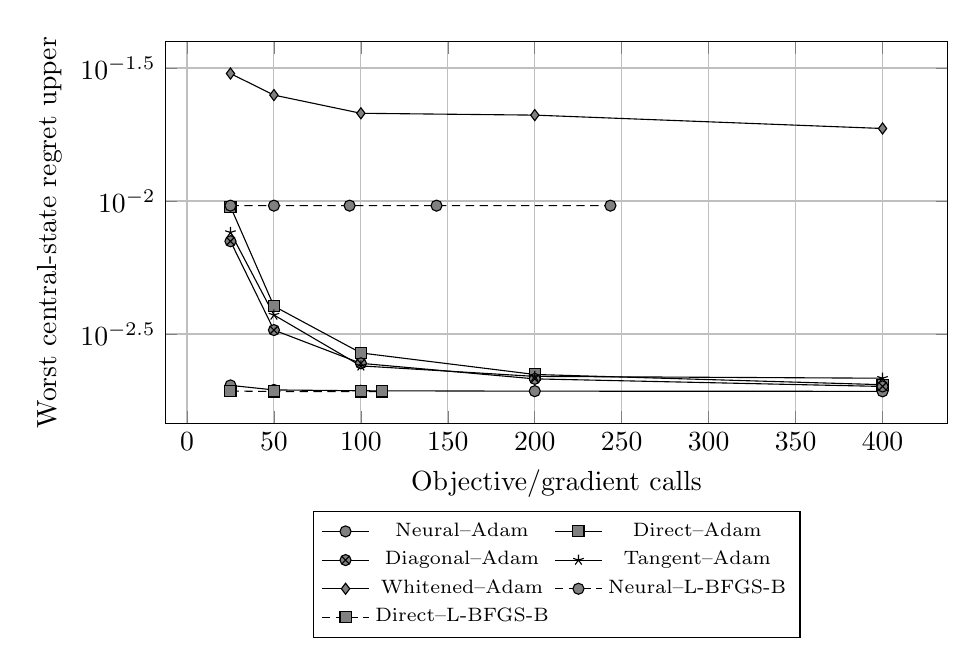
\begin{tikzpicture}\begin{axis}[width=.95\textwidth,height=.53\textwidth,ymode=log,xlabel={Objective/gradient calls},ylabel={Worst central-state regret upper},legend style={font=\scriptsize,at={(0.5,-0.23)},anchor=north,legend columns=2},cycle list name=black white,grid=major]
\addplot+ coordinates {(25,0.00202723548536) (50,0.00194949735872) (100,0.00193488823121) (200,0.00192861229754) (400,0.00192570475209)};\addlegendentry{Neural--Adam}
\addplot+ coordinates {(25,0.00952662525676) (50,0.00402452791078) (100,0.00268447423418) (200,0.00222815961052) (400,0.0020391880294)};\addlegendentry{Direct--Adam}
\addplot+ coordinates {(25,0.00706010725647) (50,0.00327279834644) (100,0.00245378270683) (200,0.00214488965772) (400,0.00200870060725)};\addlegendentry{Diagonal--Adam}
\addplot+ coordinates {(25,0.00761875768147) (50,0.00372953127525) (100,0.00239987631014) (200,0.00219158480394) (400,0.00215718190969)};\addlegendentry{Tangent--Adam}
\addplot+ coordinates {(25,0.0301533002236) (50,0.0250231010271) (100,0.0213767695895) (200,0.0210372187856) (400,0.0187422670181)};\addlegendentry{Whitened--Adam}
\addplot+ coordinates {(25,0.00960965762784) (50,0.00960818012021) (93.5,0.00960818012021) (143.5,0.00960818012021) (243.5,0.00960818012021)};\addlegendentry{Neural--L-BFGS-B}
\addplot+ coordinates {(25,0.00193053282688) (50,0.00192366681516) (100,0.00192366681516) (112,0.00192366681516) (112,0.00192366681516)};\addlegendentry{Direct--L-BFGS-B}
\end{axis}\end{tikzpicture}
\caption{All five prospective checkpoints, rule 12/24. Ordinate: worse regret bound across two seeds; abscissa: mean actual calls or cost. Lines connect recorded checkpoints, not extra observations. Certification is serial replay, so cumulative cost is reconstructed rather than directly timed online wall time.}\end{figure}
\begin{figure}[p]\centering
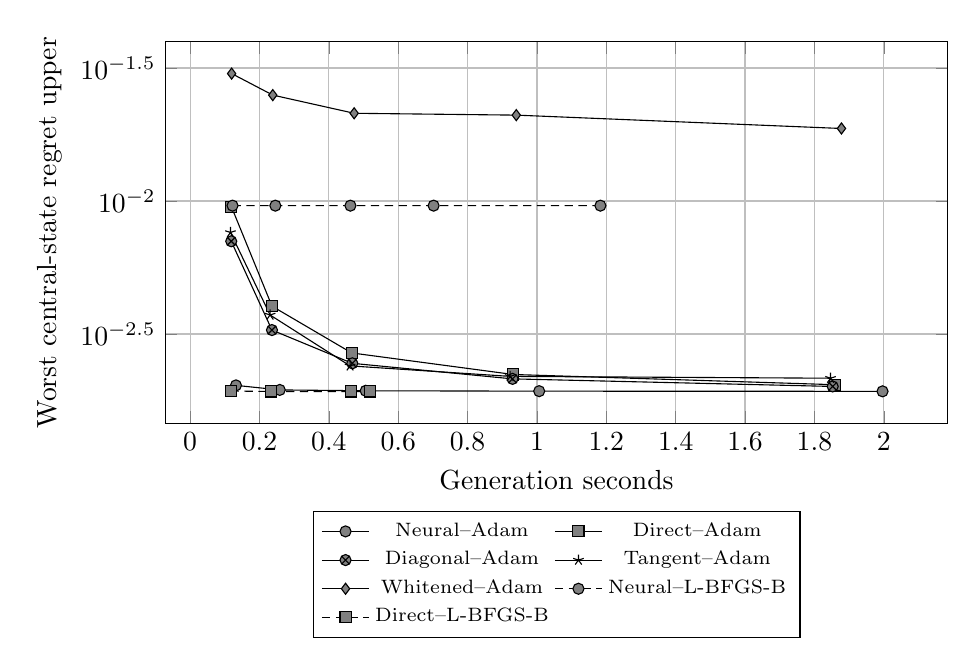
\begin{tikzpicture}\begin{axis}[width=.95\textwidth,height=.53\textwidth,ymode=log,xlabel={Generation seconds},ylabel={Worst central-state regret upper},legend style={font=\scriptsize,at={(0.5,-0.23)},anchor=north,legend columns=2},cycle list name=black white,grid=major]
\addplot+ coordinates {(0.132140211,0.00202723548536) (0.2584085655,0.00194949735872) (0.5062139445,0.00193488823121) (1.0064700815,0.00192861229754) (1.996421088,0.00192570475209)};\addlegendentry{Neural--Adam}
\addplot+ coordinates {(0.118965893,0.00952662525676) (0.236075299,0.00402452791078) (0.4659269885,0.00268447423418) (0.930847039,0.00222815961052) (1.8593667705,0.0020391880294)};\addlegendentry{Direct--Adam}
\addplot+ coordinates {(0.118510522,0.00706010725647) (0.235960516,0.00327279834644) (0.467579756,0.00245378270683) (0.9295740365,0.00214488965772) (1.8527011025,0.00200870060725)};\addlegendentry{Diagonal--Adam}
\addplot+ coordinates {(0.1163361705,0.00761875768147) (0.2305515475,0.00372953127525) (0.461180043,0.00239987631014) (0.9228222955,0.00219158480394) (1.8465210605,0.00215718190969)};\addlegendentry{Tangent--Adam}
\addplot+ coordinates {(0.1196576055,0.0301533002236) (0.238325145,0.0250231010271) (0.4730117845,0.0213767695895) (0.940394887,0.0210372187856) (1.878009586,0.0187422670181)};\addlegendentry{Whitened--Adam}
\addplot+ coordinates {(0.122253171,0.00960965762784) (0.2457344405,0.00960818012021) (0.4622194655,0.00960818012021) (0.7020173285,0.00960818012021) (1.182989959,0.00960818012021)};\addlegendentry{Neural--L-BFGS-B}
\addplot+ coordinates {(0.116861372,0.00193053282688) (0.2337607595,0.00192366681516) (0.464467812,0.00192366681516) (0.5194622975,0.00192366681516) (0.5194622975,0.00192366681516)};\addlegendentry{Direct--L-BFGS-B}
\end{axis}\end{tikzpicture}
\caption{All five prospective checkpoints, rule 12/24. Ordinate: worse regret bound across two seeds; abscissa: mean actual calls or cost. Lines connect recorded checkpoints, not extra observations. Certification is serial replay, so cumulative cost is reconstructed rather than directly timed online wall time.}\end{figure}
\begin{figure}[p]\centering
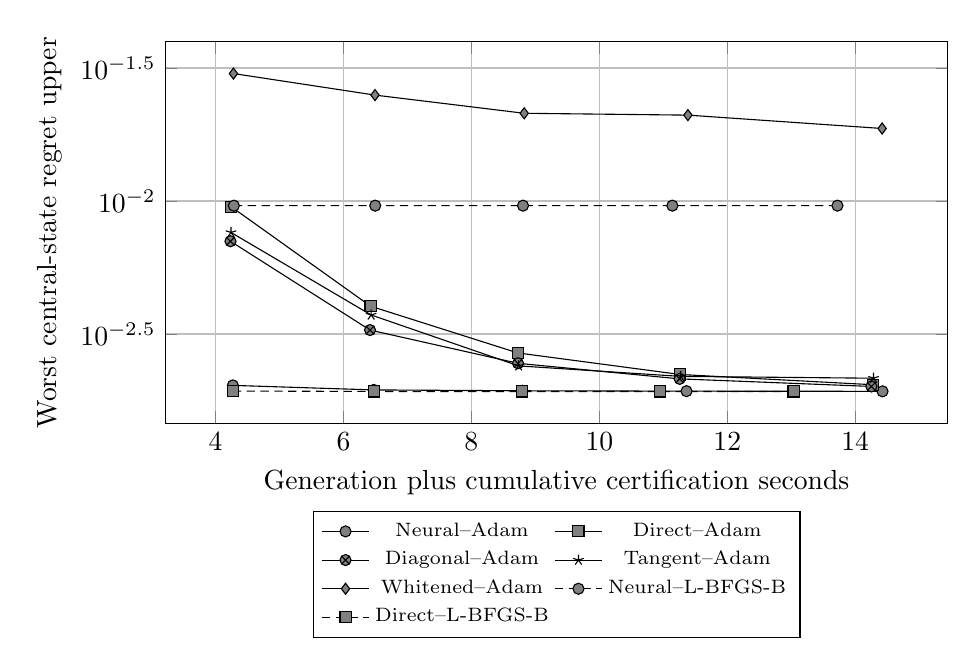
\begin{tikzpicture}\begin{axis}[width=.95\textwidth,height=.53\textwidth,ymode=log,xlabel={Generation plus cumulative certification seconds},ylabel={Worst central-state regret upper},legend style={font=\scriptsize,at={(0.5,-0.23)},anchor=north,legend columns=2},cycle list name=black white,grid=major]
\addplot+ coordinates {(4.2705961555,0.00202723548536) (6.473664638,0.00194949735872) (8.795292758,0.00193488823121) (11.362631499,0.00192861229754) (14.4270221715,0.00192570475209)};\addlegendentry{Neural--Adam}
\addplot+ coordinates {(4.2429324415,0.00952662525676) (6.4232041965,0.00402452791078) (8.7257641485,0.00268447423418) (11.259126115,0.00222815961052) (14.271826742,0.0020391880294)};\addlegendentry{Direct--Adam}
\addplot+ coordinates {(4.233464293,0.00706010725647) (6.4151471165,0.00327279834644) (8.728809561,0.00245378270683) (11.256166668,0.00214488965772) (14.252839068,0.00200870060725)};\addlegendentry{Diagonal--Adam}
\addplot+ coordinates {(4.241808324,0.00761875768147) (6.432651825,0.00372953127525) (8.7384599605,0.00239987631014) (11.2732980455,0.00219158480394) (14.2860555285,0.00215718190969)};\addlegendentry{Tangent--Adam}
\addplot+ coordinates {(4.2798077365,0.0301533002236) (6.4928988485,0.0250231010271) (8.8257559755,0.0213767695895) (11.3847944025,0.0210372187856) (14.420283594,0.0187422670181)};\addlegendentry{Whitened--Adam}
\addplot+ coordinates {(4.2865569025,0.00960965762784) (6.496318939,0.00960818012021) (8.806823538,0.00960818012021) (11.141311786,0.00960818012021) (13.7219659985,0.00960818012021)};\addlegendentry{Neural--L-BFGS-B}
\addplot+ coordinates {(4.269974264,0.00193053282688) (6.481916768,0.00192366681516) (8.794951505,0.00192366681516) (10.946349913,0.00192366681516) (13.036500431,0.00192366681516)};\addlegendentry{Direct--L-BFGS-B}
\end{axis}\end{tikzpicture}
\caption{All five prospective checkpoints, rule 12/24. Ordinate: worse regret bound across two seeds; abscissa: mean actual calls or cost. Lines connect recorded checkpoints, not extra observations. Certification is serial replay, so cumulative cost is reconstructed rather than directly timed online wall time.}\end{figure}


\clearpage
\section{Complete configuration ledger}\small
\begin{longtable}{llrrrrr}\toprule Dataset & Arm/rate & Seed & Calls & Gen. s & Check s & Candidate bound\\\midrule\endhead
tuning & Diagonal--Adam/0.005 & 24001 & 200 & 0.590 & 2.082 & 0.01691209\\
tuning & Diagonal--Adam/0.02 & 24001 & 200 & 0.612 & 2.113 & 0.003987860\\
tuning & Diagonal--Adam/0.08 & 24001 & 200 & 0.599 & 2.089 & 0.002148714\\
tuning & Direct--Adam/0.005 & 24001 & 200 & 0.593 & 2.053 & 0.01915781\\
tuning & Direct--Adam/0.02 & 24001 & 200 & 0.586 & 2.057 & 0.004725880\\
tuning & Direct--Adam/0.08 & 24001 & 200 & 0.605 & 2.065 & 0.002225349\\
tuning & Neural--Adam/0.005 & 24001 & 200 & 0.659 & 2.049 & 0.002210394\\
tuning & Neural--Adam/0.02 & 24001 & 200 & 0.654 & 2.079 & 0.001964497\\
tuning & Neural--Adam/0.08 & 24001 & 200 & 0.658 & 2.067 & 0.001927726\\
tuning & Tangent--Adam/0.005 & 24001 & 200 & 0.587 & 2.066 & 0.007097344\\
tuning & Tangent--Adam/0.02 & 24001 & 200 & 0.590 & 2.092 & 0.002566933\\
tuning & Tangent--Adam/0.08 & 24001 & 200 & 0.592 & 2.075 & 0.002049251\\
tuning & Whitened--Adam/0.005 & 24001 & 200 & 0.587 & 2.053 & 0.03177225\\
tuning & Whitened--Adam/0.02 & 24001 & 200 & 0.588 & 2.059 & 0.02071565\\
tuning & Whitened--Adam/0.08 & 24001 & 200 & 0.590 & 2.065 & 0.01775094\\
tuning & Diagonal--Adam/0.005 & 24002 & 200 & 0.589 & 2.060 & 0.01820277\\
tuning & Diagonal--Adam/0.02 & 24002 & 200 & 0.588 & 2.063 & 0.004390295\\
tuning & Diagonal--Adam/0.08 & 24002 & 200 & 0.593 & 2.067 & 0.002188804\\
tuning & Direct--Adam/0.005 & 24002 & 200 & 0.591 & 2.059 & 0.01960521\\
tuning & Direct--Adam/0.02 & 24002 & 200 & 0.589 & 2.088 & 0.004771570\\
tuning & Direct--Adam/0.08 & 24002 & 200 & 0.592 & 2.066 & 0.002228170\\
tuning & Neural--Adam/0.005 & 24002 & 200 & 0.657 & 2.073 & 0.002236912\\
tuning & Neural--Adam/0.02 & 24002 & 200 & 0.655 & 2.073 & 0.001970312\\
tuning & Neural--Adam/0.08 & 24002 & 200 & 0.661 & 2.078 & 0.001928848\\
tuning & Tangent--Adam/0.005 & 24002 & 200 & 0.588 & 2.057 & 0.009563505\\
tuning & Tangent--Adam/0.02 & 24002 & 200 & 0.592 & 2.075 & 0.003215310\\
tuning & Tangent--Adam/0.08 & 24002 & 200 & 0.598 & 2.060 & 0.002110697\\
tuning & Whitened--Adam/0.005 & 24002 & 200 & 0.587 & 2.050 & 0.02985379\\
tuning & Whitened--Adam/0.02 & 24002 & 200 & 0.589 & 2.073 & 0.02241046\\
tuning & Whitened--Adam/0.08 & 24002 & 200 & 0.594 & 2.075 & 0.02103428\\
heldout & Diagonal--Adam & 24101 & 400 & 1.855 & 10.365 & 0.002008701\\
heldout & Direct--Adam & 24101 & 400 & 1.857 & 10.384 & 0.002038210\\
heldout & Direct--L-BFGS-B & 24101 & 114 & 0.538 & 10.542 & 0.001923288\\
heldout & Neural--Adam & 24101 & 400 & 2.002 & 10.367 & 0.001925327\\
heldout & Neural--L-BFGS-B & 24101 & 87 & 0.437 & 10.580 & 0.009608170\\
heldout & Tangent--Adam & 24101 & 400 & 1.862 & 10.389 & 0.002084464\\
heldout & Whitened--Adam & 24101 & 400 & 1.918 & 10.584 & 0.01874227\\
heldout & Diagonal--Adam & 24101 & 400 & 1.182 & 10.320 & 0.002008735\\
heldout & Direct--Adam & 24101 & 400 & 1.179 & 10.325 & 0.002038249\\
heldout & Direct--L-BFGS-B & 24101 & 104 & 0.299 & 10.435 & 0.001923296\\
heldout & Neural--Adam & 24101 & 400 & 1.305 & 10.310 & 0.001925340\\
heldout & Neural--L-BFGS-B & 24101 & 102 & 0.322 & 10.452 & 0.009608291\\
heldout & Tangent--Adam & 24101 & 400 & 1.173 & 10.328 & 0.002084499\\
heldout & Whitened--Adam & 24101 & 400 & 1.172 & 10.412 & 0.01874203\\
heldout & Diagonal--Adam & 24102 & 400 & 1.851 & 10.310 & 0.002002481\\
heldout & Direct--Adam & 24102 & 400 & 1.861 & 10.321 & 0.002039189\\
heldout & Direct--L-BFGS-B & 24102 & 110 & 0.502 & 10.371 & 0.001923288\\
heldout & Neural--Adam & 24102 & 400 & 1.991 & 10.374 & 0.001925705\\
heldout & Neural--L-BFGS-B & 24102 & 400 & 1.930 & 10.378 & 0.001923323\\
heldout & Tangent--Adam & 24102 & 400 & 1.831 & 10.365 & 0.002157182\\
heldout & Whitened--Adam & 24102 & 400 & 1.838 & 10.375 & 0.01753457\\
heldout & Diagonal--Adam & 24102 & 400 & 1.176 & 10.341 & 0.002002522\\
heldout & Direct--Adam & 24102 & 400 & 1.182 & 10.500 & 0.002039228\\
heldout & Direct--L-BFGS-B & 24102 & 119 & 0.343 & 10.365 & 0.001923296\\
heldout & Neural--Adam & 24102 & 400 & 1.300 & 10.448 & 0.001925713\\
heldout & Neural--L-BFGS-B & 24102 & 400 & 1.262 & 10.505 & 0.001923374\\
heldout & Tangent--Adam & 24102 & 400 & 1.177 & 10.339 & 0.002157232\\
heldout & Whitened--Adam & 24102 & 400 & 1.178 & 10.343 & 0.01753422\\
multicell & Direct--Adam & 24300 & 400 & 1.171 & 2.071 & 0.002708729\\
multicell & Direct--L-BFGS-B & 24300 & 46 & 0.133 & 2.069 & 0.002587160\\
multicell & Neural--Adam & 24300 & 400 & 1.310 & 2.066 & 0.002589305\\
multicell & Tangent--Adam & 24300 & 400 & 1.181 & 2.073 & 0.002692616\\
multicell & Direct--Adam & 24301 & 400 & 1.168 & 2.074 & 0.002613148\\
multicell & Direct--L-BFGS-B & 24301 & 161 & 0.463 & 2.072 & 0.002488112\\
multicell & Neural--Adam & 24301 & 400 & 1.312 & 2.077 & 0.002491675\\
multicell & Tangent--Adam & 24301 & 400 & 1.169 & 2.070 & 0.002676525\\
multicell & Direct--Adam & 24302 & 400 & 1.168 & 2.088 & 0.004398790\\
multicell & Direct--L-BFGS-B & 24302 & 181 & 0.519 & 2.105 & 0.004274863\\
multicell & Neural--Adam & 24302 & 400 & 1.299 & 2.076 & 0.004280526\\
multicell & Tangent--Adam & 24302 & 400 & 1.164 & 2.074 & 0.004508256\\
multicell & Direct--Adam & 24303 & 400 & 1.170 & 2.083 & 0.002379978\\
multicell & Direct--L-BFGS-B & 24303 & 84 & 0.243 & 2.073 & 0.002267456\\
multicell & Neural--Adam & 24303 & 400 & 1.308 & 2.119 & 0.002270649\\
multicell & Tangent--Adam & 24303 & 400 & 1.168 & 2.071 & 0.002440554\\
multicell & Direct--Adam & 24304 & 400 & 1.176 & 2.066 & 0.002145888\\
multicell & Direct--L-BFGS-B & 24304 & 202 & 0.579 & 2.072 & 0.002030298\\
multicell & Neural--Adam & 24304 & 400 & 1.298 & 2.061 & 0.002036150\\
multicell & Tangent--Adam & 24304 & 400 & 1.176 & 2.075 & 0.002185028\\
multicell & Direct--Adam & 24305 & 400 & 1.178 & 2.057 & 0.003810485\\
multicell & Direct--L-BFGS-B & 24305 & 167 & 0.478 & 2.067 & 0.003696931\\
multicell & Neural--Adam & 24305 & 400 & 1.308 & 2.105 & 0.003698780\\
multicell & Tangent--Adam & 24305 & 400 & 1.166 & 2.065 & 0.003846639\\
multicell & Direct--Adam & 24306 & 400 & 1.179 & 2.063 & 0.002767600\\
multicell & Direct--L-BFGS-B & 24306 & 81 & 0.235 & 2.086 & 0.002664646\\
multicell & Neural--Adam & 24306 & 400 & 1.310 & 2.062 & 0.002667582\\
multicell & Tangent--Adam & 24306 & 400 & 1.178 & 2.077 & 0.002799149\\
multicell & Direct--Adam & 24307 & 400 & 1.173 & 2.075 & 0.002395412\\
multicell & Direct--L-BFGS-B & 24307 & 169 & 0.486 & 2.061 & 0.002288317\\
multicell & Neural--Adam & 24307 & 400 & 1.304 & 2.062 & 0.002291286\\
multicell & Tangent--Adam & 24307 & 400 & 1.177 & 2.086 & 0.002425920\\
multicell & Direct--Adam & 24308 & 400 & 1.169 & 2.062 & 0.003940201\\
multicell & Direct--L-BFGS-B & 24308 & 159 & 0.456 & 2.089 & 0.003834396\\
multicell & Neural--Adam & 24308 & 400 & 1.307 & 2.059 & 0.003837366\\
multicell & Tangent--Adam & 24308 & 400 & 1.170 & 2.069 & 0.003973639\\
reference & Diagonal--Adam & 24501 & 400 & 0.196 & 0.066 & 0.00005270608\\
reference & Direct--Adam & 24501 & 400 & 0.198 & 0.066 & 0.00005026021\\
reference & Direct--L-BFGS-B & 24501 & 14 & 0.007 & 0.067 & $3.392842\times10^{-13}$\\
reference & Neural--Adam & 24501 & 400 & 0.321 & 0.066 & 0.002771190\\
reference & Tangent--Adam & 24501 & 400 & 0.197 & 0.067 & 0.00001955686\\
reference & Whitened--Adam & 24501 & 400 & 0.196 & 0.066 & 0.5345057\\
reference & Diagonal--Adam & 24502 & 400 & 0.198 & 0.066 & 0.00006450277\\
reference & Direct--Adam & 24502 & 400 & 0.199 & 0.067 & 0.00005492341\\
reference & Direct--L-BFGS-B & 24502 & 14 & 0.007 & 0.066 & $9.192647\times10^{-14}$\\
reference & Neural--Adam & 24502 & 400 & 0.321 & 0.066 & $3.620557\times10^{-8}$\\
reference & Tangent--Adam & 24502 & 400 & 0.197 & 0.067 & $8.427595\times10^{-6}$\\
reference & Whitened--Adam & 24502 & 400 & 0.196 & 0.073 & 0.5646302\\
failure & direct restart & 23203 & 4 & 0.013 & 10.704 & 0.01050307\\
failure & regenerated & 23203 & 92 & 0.299 & 10.934 & 0.01050307\\
failure & restart tighter & 23203 & 43 & 0.141 & 10.772 & 0.01050307\\
failure & scaled & 23203 & 400 & 1.423 & 10.800 & 0.002554827\\
\bottomrule\end{longtable}\normalsize
\section{All 140 held-out checkpoints}\small
\begin{longtable}{llrrrrr}\toprule Seed/rule & Arm & Cap & Calls & Deployed bound & Gen. s & Cum. check s\\\midrule\endhead
24101/12 & Diagonal--Adam & 25 & 25 & 0.007060108 & 0.120 & 2.052\\
24101/12 & Diagonal--Adam & 50 & 50 & 0.003272799 & 0.241 & 4.128\\
24101/12 & Diagonal--Adam & 100 & 100 & 0.002453783 & 0.473 & 6.216\\
24101/12 & Diagonal--Adam & 200 & 200 & 0.002144890 & 0.937 & 8.287\\
24101/12 & Diagonal--Adam & 400 & 400 & 0.002008701 & 1.855 & 10.365\\
24101/12 & Direct--Adam & 25 & 25 & 0.009302293 & 0.119 & 2.070\\
24101/12 & Direct--Adam & 50 & 50 & 0.003987056 & 0.235 & 4.132\\
24101/12 & Direct--Adam & 100 & 100 & 0.002676558 & 0.466 & 6.212\\
24101/12 & Direct--Adam & 200 & 200 & 0.002225434 & 0.927 & 8.287\\
24101/12 & Direct--Adam & 400 & 400 & 0.002038210 & 1.857 & 10.384\\
24101/12 & Direct--L-BFGS-B & 25 & 25 & 0.001930155 & 0.118 & 2.109\\
24101/12 & Direct--L-BFGS-B & 50 & 50 & 0.001923471 & 0.238 & 4.220\\
24101/12 & Direct--L-BFGS-B & 100 & 100 & 0.001923471 & 0.473 & 6.314\\
24101/12 & Direct--L-BFGS-B & 200 & 114 & 0.001923471 & 0.538 & 8.433\\
24101/12 & Direct--L-BFGS-B & 400 & 114 & 0.001923471 & 0.538 & 10.542\\
24101/12 & Neural--Adam & 25 & 25 & 0.002001374 & 0.133 & 2.075\\
24101/12 & Neural--Adam & 50 & 50 & 0.001949498 & 0.262 & 4.156\\
24101/12 & Neural--Adam & 100 & 100 & 0.001934889 & 0.508 & 6.231\\
24101/12 & Neural--Adam & 200 & 200 & 0.001928613 & 1.012 & 8.297\\
24101/12 & Neural--Adam & 400 & 400 & 0.001925327 & 2.002 & 10.367\\
24101/12 & Neural--L-BFGS-B & 25 & 25 & 0.009609658 & 0.122 & 2.133\\
24101/12 & Neural--L-BFGS-B & 50 & 50 & 0.009608181 & 0.248 & 4.235\\
24101/12 & Neural--L-BFGS-B & 100 & 87 & 0.009608181 & 0.437 & 6.349\\
24101/12 & Neural--L-BFGS-B & 200 & 87 & 0.009608181 & 0.437 & 8.463\\
24101/12 & Neural--L-BFGS-B & 400 & 87 & 0.009608181 & 0.437 & 10.580\\
24101/12 & Tangent--Adam & 25 & 25 & 0.004484666 & 0.119 & 2.067\\
24101/12 & Tangent--Adam & 50 & 50 & 0.002390348 & 0.234 & 4.141\\
24101/12 & Tangent--Adam & 100 & 100 & 0.002139910 & 0.466 & 6.210\\
24101/12 & Tangent--Adam & 200 & 200 & 0.002095942 & 0.927 & 8.278\\
24101/12 & Tangent--Adam & 400 & 400 & 0.002084464 & 1.862 & 10.389\\
24101/12 & Whitened--Adam & 25 & 25 & 0.03015331 & 0.123 & 2.120\\
24101/12 & Whitened--Adam & 50 & 50 & 0.02360656 & 0.247 & 4.234\\
24101/12 & Whitened--Adam & 100 & 100 & 0.02025888 & 0.482 & 6.351\\
24101/12 & Whitened--Adam & 200 & 200 & 0.01892330 & 0.957 & 8.464\\
24101/12 & Whitened--Adam & 400 & 400 & 0.01874227 & 1.918 & 10.584\\
24101/8 & Diagonal--Adam & 25 & 25 & 0.007060108 & 0.075 & 2.057\\
24101/8 & Diagonal--Adam & 50 & 50 & 0.003272823 & 0.148 & 4.117\\
24101/8 & Diagonal--Adam & 100 & 100 & 0.002453835 & 0.296 & 6.185\\
24101/8 & Diagonal--Adam & 200 & 200 & 0.002144940 & 0.597 & 8.255\\
24101/8 & Diagonal--Adam & 400 & 400 & 0.002008735 & 1.182 & 10.320\\
24101/8 & Direct--Adam & 25 & 25 & 0.009302295 & 0.076 & 2.065\\
24101/8 & Direct--Adam & 50 & 50 & 0.003987081 & 0.150 & 4.137\\
24101/8 & Direct--Adam & 100 & 100 & 0.002676606 & 0.297 & 6.202\\
24101/8 & Direct--Adam & 200 & 200 & 0.002225488 & 0.591 & 8.259\\
24101/8 & Direct--Adam & 400 & 400 & 0.002038249 & 1.179 & 10.325\\
24101/8 & Direct--L-BFGS-B & 25 & 25 & 0.001930173 & 0.072 & 2.085\\
24101/8 & Direct--L-BFGS-B & 50 & 50 & 0.001923443 & 0.144 & 4.174\\
24101/8 & Direct--L-BFGS-B & 100 & 100 & 0.001923443 & 0.287 & 6.254\\
24101/8 & Direct--L-BFGS-B & 200 & 104 & 0.001923443 & 0.299 & 8.332\\
24101/8 & Direct--L-BFGS-B & 400 & 104 & 0.001923443 & 0.299 & 10.435\\
24101/8 & Neural--Adam & 25 & 25 & 0.002001375 & 0.085 & 2.059\\
24101/8 & Neural--Adam & 50 & 50 & 0.001949502 & 0.166 & 4.113\\
24101/8 & Neural--Adam & 100 & 100 & 0.001934911 & 0.330 & 6.177\\
24101/8 & Neural--Adam & 200 & 200 & 0.001928632 & 0.656 & 8.244\\
24101/8 & Neural--Adam & 400 & 400 & 0.001925340 & 1.305 & 10.310\\
24101/8 & Neural--L-BFGS-B & 25 & 25 & 0.009609672 & 0.079 & 2.102\\
24101/8 & Neural--L-BFGS-B & 50 & 50 & 0.009608327 & 0.159 & 4.190\\
24101/8 & Neural--L-BFGS-B & 100 & 100 & 0.009608327 & 0.315 & 6.278\\
24101/8 & Neural--L-BFGS-B & 200 & 102 & 0.009608327 & 0.322 & 8.364\\
24101/8 & Neural--L-BFGS-B & 400 & 102 & 0.009608327 & 0.322 & 10.452\\
24101/8 & Tangent--Adam & 25 & 25 & 0.004484680 & 0.075 & 2.058\\
24101/8 & Tangent--Adam & 50 & 50 & 0.002390433 & 0.148 & 4.124\\
24101/8 & Tangent--Adam & 100 & 100 & 0.002139947 & 0.293 & 6.187\\
24101/8 & Tangent--Adam & 200 & 200 & 0.002095993 & 0.585 & 8.248\\
24101/8 & Tangent--Adam & 400 & 400 & 0.002084499 & 1.172 & 10.328\\
24101/8 & Whitened--Adam & 25 & 25 & 0.03015330 & 0.074 & 2.062\\
24101/8 & Whitened--Adam & 50 & 50 & 0.02360656 & 0.148 & 4.158\\
24101/8 & Whitened--Adam & 100 & 100 & 0.02025888 & 0.295 & 6.220\\
24101/8 & Whitened--Adam & 200 & 200 & 0.01892319 & 0.586 & 8.318\\
24101/8 & Whitened--Adam & 400 & 400 & 0.01874203 & 1.172 & 10.412\\
24102/12 & Diagonal--Adam & 25 & 25 & 0.006559432 & 0.117 & 2.053\\
24102/12 & Diagonal--Adam & 50 & 50 & 0.003128239 & 0.231 & 4.106\\
24102/12 & Diagonal--Adam & 100 & 100 & 0.002407914 & 0.462 & 6.181\\
24102/12 & Diagonal--Adam & 200 & 200 & 0.002127916 & 0.922 & 8.241\\
24102/12 & Diagonal--Adam & 400 & 400 & 0.002002481 & 1.850 & 10.310\\
24102/12 & Direct--Adam & 25 & 25 & 0.009526626 & 0.119 & 2.058\\
24102/12 & Direct--Adam & 50 & 50 & 0.004024528 & 0.237 & 4.122\\
24102/12 & Direct--Adam & 100 & 100 & 0.002684475 & 0.466 & 6.187\\
24102/12 & Direct--Adam & 200 & 200 & 0.002228160 & 0.935 & 8.249\\
24102/12 & Direct--Adam & 400 & 400 & 0.002039189 & 1.861 & 10.321\\
24102/12 & Direct--L-BFGS-B & 25 & 25 & 0.001930533 & 0.116 & 2.077\\
24102/12 & Direct--L-BFGS-B & 50 & 50 & 0.001923667 & 0.229 & 4.156\\
24102/12 & Direct--L-BFGS-B & 100 & 100 & 0.001923667 & 0.456 & 6.226\\
24102/12 & Direct--L-BFGS-B & 200 & 110 & 0.001923667 & 0.501 & 8.300\\
24102/12 & Direct--L-BFGS-B & 400 & 110 & 0.001923667 & 0.501 & 10.371\\
24102/12 & Neural--Adam & 25 & 25 & 0.002027236 & 0.131 & 2.081\\
24102/12 & Neural--Adam & 50 & 50 & 0.001945647 & 0.254 & 4.154\\
24102/12 & Neural--Adam & 100 & 100 & 0.001933843 & 0.504 & 6.227\\
24102/12 & Neural--Adam & 200 & 200 & 0.001928228 & 1.001 & 8.295\\
24102/12 & Neural--Adam & 400 & 400 & 0.001925705 & 1.991 & 10.374\\
24102/12 & Neural--L-BFGS-B & 25 & 25 & 0.001941987 & 0.122 & 2.075\\
24102/12 & Neural--L-BFGS-B & 50 & 50 & 0.001932375 & 0.244 & 4.145\\
24102/12 & Neural--L-BFGS-B & 100 & 100 & 0.001926151 & 0.488 & 6.220\\
24102/12 & Neural--L-BFGS-B & 200 & 200 & 0.001923514 & 0.967 & 8.295\\
24102/12 & Neural--L-BFGS-B & 400 & 400 & 0.001923514 & 1.929 & 10.378\\
24102/12 & Tangent--Adam & 25 & 25 & 0.007618758 & 0.114 & 2.059\\
24102/12 & Tangent--Adam & 50 & 50 & 0.003729532 & 0.227 & 4.138\\
24102/12 & Tangent--Adam & 100 & 100 & 0.002399877 & 0.456 & 6.219\\
24102/12 & Tangent--Adam & 200 & 200 & 0.002191585 & 0.918 & 8.298\\
24102/12 & Tangent--Adam & 400 & 400 & 0.002157182 & 1.831 & 10.365\\
24102/12 & Whitened--Adam & 25 & 25 & 0.02925194 & 0.116 & 2.075\\
24102/12 & Whitened--Adam & 50 & 50 & 0.02502311 & 0.230 & 4.150\\
24102/12 & Whitened--Adam & 100 & 100 & 0.02137677 & 0.464 & 6.230\\
24102/12 & Whitened--Adam & 200 & 200 & 0.02103722 & 0.924 & 8.299\\
24102/12 & Whitened--Adam & 400 & 400 & 0.01753457 & 1.838 & 10.375\\
24102/8 & Diagonal--Adam & 25 & 25 & 0.006559436 & 0.073 & 2.047\\
24102/8 & Diagonal--Adam & 50 & 50 & 0.003128267 & 0.148 & 4.124\\
24102/8 & Diagonal--Adam & 100 & 100 & 0.002407976 & 0.295 & 6.212\\
24102/8 & Diagonal--Adam & 200 & 200 & 0.002127976 & 0.588 & 8.278\\
24102/8 & Diagonal--Adam & 400 & 400 & 0.002002522 & 1.176 & 10.341\\
24102/8 & Direct--Adam & 25 & 25 & 0.009526628 & 0.074 & 2.101\\
24102/8 & Direct--Adam & 50 & 50 & 0.004024553 & 0.147 & 4.203\\
24102/8 & Direct--Adam & 100 & 100 & 0.002684523 & 0.296 & 6.318\\
24102/8 & Direct--Adam & 200 & 200 & 0.002228214 & 0.590 & 8.427\\
24102/8 & Direct--Adam & 400 & 400 & 0.002039228 & 1.182 & 10.500\\
24102/8 & Direct--L-BFGS-B & 25 & 25 & 0.001930543 & 0.073 & 2.075\\
24102/8 & Direct--L-BFGS-B & 50 & 50 & 0.001923689 & 0.144 & 4.143\\
24102/8 & Direct--L-BFGS-B & 100 & 100 & 0.001923297 & 0.288 & 6.217\\
24102/8 & Direct--L-BFGS-B & 200 & 119 & 0.001923297 & 0.343 & 8.288\\
24102/8 & Direct--L-BFGS-B & 400 & 119 & 0.001923297 & 0.343 & 10.365\\
24102/8 & Neural--Adam & 25 & 25 & 0.002027461 & 0.085 & 2.110\\
24102/8 & Neural--Adam & 50 & 50 & 0.001945621 & 0.167 & 4.203\\
24102/8 & Neural--Adam & 100 & 100 & 0.001933842 & 0.329 & 6.291\\
24102/8 & Neural--Adam & 200 & 200 & 0.001928233 & 0.651 & 8.372\\
24102/8 & Neural--Adam & 400 & 400 & 0.001925713 & 1.300 & 10.448\\
24102/8 & Neural--L-BFGS-B & 25 & 25 & 0.001942199 & 0.079 & 2.070\\
24102/8 & Neural--L-BFGS-B & 50 & 50 & 0.001932827 & 0.160 & 4.161\\
24102/8 & Neural--L-BFGS-B & 100 & 100 & 0.001924547 & 0.317 & 6.314\\
24102/8 & Neural--L-BFGS-B & 200 & 200 & 0.001923533 & 0.631 & 8.425\\
24102/8 & Neural--L-BFGS-B & 400 & 400 & 0.001923533 & 1.261 & 10.505\\
24102/8 & Tangent--Adam & 25 & 25 & 0.007618825 & 0.074 & 2.069\\
24102/8 & Tangent--Adam & 50 & 50 & 0.003729551 & 0.148 & 4.136\\
24102/8 & Tangent--Adam & 100 & 100 & 0.002399927 & 0.295 & 6.205\\
24102/8 & Tangent--Adam & 200 & 200 & 0.002191637 & 0.588 & 8.263\\
24102/8 & Tangent--Adam & 400 & 400 & 0.002157232 & 1.177 & 10.339\\
24102/8 & Whitened--Adam & 25 & 25 & 0.02925194 & 0.073 & 2.051\\
24102/8 & Whitened--Adam & 50 & 50 & 0.02502295 & 0.148 & 4.109\\
24102/8 & Whitened--Adam & 100 & 100 & 0.02137650 & 0.294 & 6.174\\
24102/8 & Whitened--Adam & 200 & 200 & 0.02103689 & 0.590 & 8.242\\
24102/8 & Whitened--Adam & 400 & 400 & 0.01753422 & 1.178 & 10.343\\
\bottomrule\end{longtable}\normalsize


\section{Machine-readable evidence and reproduction}
\path{results/COMPLETE_LEDGER.json} and its CSV version enumerate all 110 trajectories. \path{results/CHECKPOINT_LEDGER.json} and CSV enumerate all 286 checkpoints, including acceptance flags omitted from the narrower printed table. Per-run records retain raw policies, dyadic coefficients, initial and deployed certificates, call counts, objective/gradient histories, termination, generation and checking times. Held-out checkpoints additionally include both proposal gradients, pricing offsets and actual Jacobian singular values.

\path{results/DEPENDENCY_LOCK.json} identifies runtime-imported repository modules and inherited numerical data with SHA-256 hashes. \path{PUBLICATION_MANIFEST.json} additionally locks transitive TeX inputs, all R24 evidence and the final PDFs. \path{results/PRIMARY_EVIDENCE_LOCK.json} verifies the recovered primary bytes, and \path{results/PRESERVATION_AUDIT.json} verifies every file inherited from the reviewed branch. The publication manifest and enclosing source archive are excluded from their own hash lists to avoid self-reference.

\path{results/full_state_canonical.json} is the current schema-version-two interpretation of the full-state record. It identifies the discounted all-start-time bound 7.241462443133396 and preserves the old undiscounted quantity as historical. No old summary is overwritten, and no new full-state policy improvement is recorded.

From the repository root, run \path{replication/assemble_publication.py} within the R24 revision folder, then build \path{ECTA_R24.tex}, \path{SUPP_R24.tex} and \path{RESPONSE_R24.tex}. This regenerates publication tables from frozen evidence, not new optimization. Fresh scientific regeneration uses a disposable checkout, retains the original results elsewhere, and runs \path{study.py --phase all} in the locked numerical environment. The complete commands in \path{REPRODUCE.md} and the manual reproduction workflow keep fresh results separate from the published evidence.
